\documentclass[11pt,]{article}
\usepackage{lmodern}
\usepackage{amssymb,amsmath}
\usepackage{ifxetex,ifluatex}
\usepackage{fixltx2e} % provides \textsubscript
\ifnum 0\ifxetex 1\fi\ifluatex 1\fi=0 % if pdftex
  \usepackage[T1]{fontenc}
  \usepackage[utf8]{inputenc}
\else % if luatex or xelatex
  \ifxetex
    \usepackage{mathspec}
  \else
    \usepackage{fontspec}
  \fi
  \defaultfontfeatures{Ligatures=TeX,Scale=MatchLowercase}
\fi
% use upquote if available, for straight quotes in verbatim environments
\IfFileExists{upquote.sty}{\usepackage{upquote}}{}
% use microtype if available
\IfFileExists{microtype.sty}{%
\usepackage{microtype}
\UseMicrotypeSet[protrusion]{basicmath} % disable protrusion for tt fonts
}{}
\usepackage[margin=1.0in]{geometry}
\usepackage{hyperref}
\hypersetup{unicode=true,
            pdfborder={0 0 0},
            breaklinks=true}
\urlstyle{same}  % don't use monospace font for urls
\usepackage{graphicx,grffile}
\makeatletter
\def\maxwidth{\ifdim\Gin@nat@width>\linewidth\linewidth\else\Gin@nat@width\fi}
\def\maxheight{\ifdim\Gin@nat@height>\textheight\textheight\else\Gin@nat@height\fi}
\makeatother
% Scale images if necessary, so that they will not overflow the page
% margins by default, and it is still possible to overwrite the defaults
% using explicit options in \includegraphics[width, height, ...]{}
\setkeys{Gin}{width=\maxwidth,height=\maxheight,keepaspectratio}
\IfFileExists{parskip.sty}{%
\usepackage{parskip}
}{% else
\setlength{\parindent}{0pt}
\setlength{\parskip}{6pt plus 2pt minus 1pt}
}
\setlength{\emergencystretch}{3em}  % prevent overfull lines
\providecommand{\tightlist}{%
  \setlength{\itemsep}{0pt}\setlength{\parskip}{0pt}}
\setcounter{secnumdepth}{0}
% Redefines (sub)paragraphs to behave more like sections
\ifx\paragraph\undefined\else
\let\oldparagraph\paragraph
\renewcommand{\paragraph}[1]{\oldparagraph{#1}\mbox{}}
\fi
\ifx\subparagraph\undefined\else
\let\oldsubparagraph\subparagraph
\renewcommand{\subparagraph}[1]{\oldsubparagraph{#1}\mbox{}}
\fi

%%% Use protect on footnotes to avoid problems with footnotes in titles
\let\rmarkdownfootnote\footnote%
\def\footnote{\protect\rmarkdownfootnote}

%%% Change title format to be more compact
\usepackage{titling}

% Create subtitle command for use in maketitle
\newcommand{\subtitle}[1]{
  \posttitle{
    \begin{center}\large#1\end{center}
    }
}

\setlength{\droptitle}{-2em}

  \title{}
    \pretitle{\vspace{\droptitle}}
  \posttitle{}
    \author{}
    \preauthor{}\postauthor{}
    \date{}
    \predate{}\postdate{}
  
\usepackage{helvet} % Helvetica font
\renewcommand*\familydefault{\sfdefault} % Use the sans serif version of the font
\usepackage[T1]{fontenc}

\usepackage[none]{hyphenat}

\usepackage{setspace}
\doublespacing
\setlength{\parskip}{1em}

\usepackage{lineno}

\usepackage{pdfpages}

\begin{document}

\vspace{35mm}

\hypertarget{fecal-short-chain-fatty-acids-are-not-predictive-of-colonic-tumor-status-and-cannot-be-predicted-based-on-bacterial-community-structure}{%
\section{Fecal short chain fatty acids are not predictive of colonic
tumor status and cannot be predicted based on bacterial community
structure}\label{fecal-short-chain-fatty-acids-are-not-predictive-of-colonic-tumor-status-and-cannot-be-predicted-based-on-bacterial-community-structure}}

\vspace{35mm}

Marc A. Sze\({^1}\), Begüm D. Topçuoğlu\({^1}\), Nicholas A.
Lesniak\({^1}\), Mack T. Ruffin IV\({^2}\), Patrick D.
Schloss\({^1}\)\({^\dagger}\)

\vspace{40mm}

\(\dagger\) To whom correspondence should be addressed:
\href{mailto:pschloss@umich.edu}{\nolinkurl{pschloss@umich.edu}}

\(1\) Department of Microbiology and Immunology, University of Michigan,
Ann Arbor, MI 48109

\(2\) Department of Family Medicine and Community Medicine, Penn State
Hershey Medical Center, Hershey, PA

\vspace{10mm}

\hypertarget{observation-format}{%
\subsection{Observation format}\label{observation-format}}

\newpage
\linenumbers

\hypertarget{abstract}{%
\subsection{Abstract}\label{abstract}}

Colonic bacterial populations are thought to have a role in the
development of colorectal cancer with some protecting against
inflammation and others exacerbating inflammation. Short chain fatty
acids (SCFAs), including butyrate, have been shown to have
anti-inflammatory properties and are produced in large quantities by
colonic bacteria which produce SCFAs by fermenting fiber. We assessed
whether there was an association between fecal SCFA concentrations and
the presence of colonic adenomas or carcinomas in a cohort of
individuals using 16S rRNA gene and metagenomic shotgun sequence data.
We measured the fecal concentrations of acetate, propionate, and
butyrate within the cohort and found that there were no significant
associations between SCFA concentration and disease status. When we
incorporated these concentrations into random forest classification
models trained to differentiate between people with normal colons and
those with adenomas or carcinomas, we found that they did not
significantly improve the ability of 16S rRNA gene or metagenomic gene
sequence-based models to classify individuals. Finally, we generated
random forest regression models trained to predict the concentration of
each SCFA based on 16S rRNA gene or metagenomic gene sequence data from
the same samples. These models performed poorly and were able to explain
at most 14\% of the observed variation in the SCFA concentrations. These
results support the broader epidemiological data that questions the
value of fiber consumption for reducing the risks of colorectal cancer.
Although other bacterial metabolites may serve as biomarkers to detect
adenomas or carcinomas, fecal SCFA concentrations have limited
predictive power.

\newpage

\hypertarget{importance}{%
\subsection{Importance}\label{importance}}

Considering colorectal cancer is the third leading cancer-related cause
of death within the United States, there is a great need to detect
colorectal tumors early without invasive colonoscopy procedures and to
prevent the formation of tumors. Short chain fatty acids (SCFAs) are
often used as a surrogate for measuring gut health and for being
anti-carcinogenic because of their anti-inflammatory properties. We
evaluated the fecal SCFA concentration of a cohort of individuals with
varying colonic tumor burden who were previously analyzed to identify
microbiome-based biomarkers of tumors. We were unable to find an
association between SCFA concentration and tumor burden or use SCFAs to
improve our microbiome-based models of classifying people based on their
tumor status. Furthermore, we were unable to find an association between
the fecal community structure and SCFA concentrations. These data
indicate that there is no conclusive link between the gut microbiome,
SCFAs, and tumor burden.

\newpage

Colorectal cancer is the third leading cancer-related cause of death
within the United States (1). Less than 10\% of cases can be attributed
to genetic risk factors (2). This leaves a significant role for
environmental and behavioral factors and diet (3, 4). Colorectal cancer
is thought to be initiated by a series of mutations that accumulate as
the mutated cells begin to proliferate leading to adenomatous lesions,
which are succeeded by carcinomas (2). Throughout this progression,
there are ample opportunities for bacterial populations to have a role
as bacteria are known to cause mutations, induce inflammation, and
accelerate tumorigenesis (5--7). Additional cross sectional studies in
humans have identified microbiome-based biomarkers of disease (8). These
studies suggest that in some cases, it is the loss of bacterial
populations that produce short-chain fatty acids (SCFAs) that results in
increased inflammation and tumorigenesis.

Many microbiome studies use the concentrations of SCFAs and the presence
of 16S rRNA gene sequences from organisms and the genes involved in
producing them as a biomarker of a healthy microbiota (9, 10). SCFAs
have anti-inflammatory and anti-proliferative activities (11). Direct
supplementation of SCFAs or feeding of fiber caused an overall reduction
in tumor burden in mouse models of colorectal cancer (12). These results
suggest that supplementation with fiber, which many colonic bacteria
ferment to produce SCFAs may confer beneficial effects against
colorectal cancer. Regardless, there is a lack of evidence that
increasing SCFA concentrations can protect against colorectal cancer in
humans. Case-control studies that have investigated possible
associations between SCFAs and colon tumor status have been plagued by
relatively small numbers of subjects, but have reported increased total
and relative fecal acetate levels and decreased relative fecal butyrate
concentrations in subjects with colonic lesions (13). In randomized
controlled trials fiber supplementation has been inconsistently
associated with protection against tumor formation and recurrence (14,
15). These findings temper enthusiasm for treatments that aim to use
SCFAs as biomarkers or protection against tumorigenesis.

\textbf{Fecal SCFA concentrations did not vary with diagnosis or
treatment.} To quantify the associations between colorectal cancer, the
microbiome, and SCFAs, we quantified the concentration of acetate,
propionate, and butyrate in feces of previously characterized
individuals with normal colons (N=172) and those with colonic adenomas
(N=198) or carcinomas (N=120) (16). We were unable to detect a
significant difference in any SCFA concentration across the diagnoses
groups (all P\textgreater{}0.15; Figure 1A). Among the individuals with
adenomas and carcinomas, a subset (N\textsubscript{adenoma}=41,
N\textsubscript{carcinoma}=26) were treated and sampled a year later
(17). None of the SCFAs exhibited a significant change with treatment
(all P\textgreater{}0.058; Figure 1B). For both the pre-treatment
cross-sectional data and the pre/post treatment data, we also failed to
detect any significant differences in the relative concentrations of any
SCFAs (P\textgreater{}0.16). Finally, we pooled the SCFA concentrations
on a total and per molecule of carbon basis and again failed to observe
any significant differences (P\textgreater{}0.077). These results
demonstrated that there were no significant associations between fecal
SCFA concentration and diagnosis or treatment.

\textbf{Combining SCFA and microbiome data does not improve the ability
to diagnose individual as having adenomas or carcinomas.} We previously
found that binning 16S rRNA gene sequence data into operational
taxonomic units (OTUs) based on 97\% similarity or into genera enabled
us to classify individuals as having adenomas or carcinomas using random
forest machine learning models (8, 16). We repeated that analysis but
added the concentration of the SCFAs as possible features to train the
models (Figure S1). Models trained using SCFAs to classify individuals
as having adenomas or carcinomas rather than normal colons had median
areas under the receiver operator characteristic curve (AUROC) that were
significantly greater than 0.5 (P\textsubscript{adenoma}\textless{}0.001
and P\textsubscript{carcinoma}\textless{}0.001). However, the AUROC
values to detect the presence of adenomas or carcinomas were only 0.54
and 0.55, respectively, indicating that SCFAs had poor predictive power
on their own (Figure 2A). When we trained the models with the SCFAs
concentrations and OTU or genus-level relative abundances the AUROC
values were not significantly different from the same models trained
without the SCFA concentrations (P\textgreater{}0.21; Figure 2A). These
data demonstrate that knowledge of the SCFA profile from a patient's
fecal sample did not improve the ability to diagnose a colonic lesion.

\textbf{Knowledge of microbial community structure does not predict SCFA
concentrations.} We next asked whether the fecal community structure was
predictive of fecal SCFA concentrations, regardless of a person's
diagnosis. We trained random forest regression models using 16S rRNA
gene sequence data binned into OTUs and genera to predict the
concentration of the SCFAs (Figure S2). The largest R\textsuperscript{2}
between the observed SCFA concentrations and the modeled concentrations
was 0.14, which was observed when using genus data to predict butyrate
concentrations (Figure 2B). We also used a smaller dataset of shotgun
metagenomic sequencing data generated from a subset of our cohort
(N\textsubscript{normal}=27, N\textsubscript{adenoma}=25, and
N\textsubscript{cancer}=26) (18). We binned genes extracted from the
assembled metagenomes into operational protein families (OPFs) or KEGG
categories and trained random forest regression models using metagenomic
sequence data to predict the concentration of the SCFAs (Figure S2).
Similar to the analysis using 16S rRNA gene sequence data, the
metagenomic data was not predictive of SCFA concentration; the largest
amount of variation that the models could explain was 5.45\%, which was
observed when using KEGG data to predict propionate concentrations
(Figure 2B). Because of the limited number of samples that we were able
to generate metagenomic sequence data from, we used our 16S rRNA gene
sequence data to impute metagenomes that were binned into metabolic
pathways or KEGG categories using PICRUSt (Figure S2). SCFA
concentrations could not be predicted based on the imputed metagenomic
data. The largest amount of variation that the models could explain was
9.67\%, which was observed when using KEGG data to predict butyrate
concentrations (Figure 2B). The inability to model SCFA concentrations
from microbiome data indicates that the knowledge of the abundance of
organisms and their genes was insufficient to predict SCFA
concentrations.

\textbf{Conclusion.} Our data indicate that fecal SCFA concentrations
are not associated with the presence of adenomas or carcinomas and that
they provide weak predictive power to improve the ability to diagnose
someone with one of these lesions. Furthermore, knowledge of the
taxonomic and genetic structure of gut microbiota was not predictive of
SCFA concentrations. These results complement existing literature that
suggest that fiber consumption and the production of SCFAs are unable to
prevent the risk of developing colonic tumors. It is important to note
that our analysis concerned fecal SCFA concentrations and microbiome
characterization and that observations along the mucosa near the site of
lesions may provide a stronger association. Regardless, given the
growing literature in this area, it is unlikely that SCFAs are the
primary mechanism that limits tumorigenesis. This may be a cautionary
result to temper enthusiasm for SCFAs as a biomarker of gut health more
generally. Going forward it is critical to develop additional hypotheses
for how the microbiome and host interact to drive tumorigenesis so that
we can better understand tumorigenesis and identify biomarkers that will
allow early detection of lesions.

\hypertarget{acknowledgements}{%
\subsection{Acknowledgements}\label{acknowledgements}}

The authors thank the Great Lakes-New England Early Detection Research
Network for providing the fecal samples that were used in this study. We
would thank the University of Michigan Center for Microbial Systems for
enabling our short-chain fatty acid analysis. Support for MAS came from
the Canadian Institute of Health Research and the National Institutes of
Health (UL1TR002240). This work was also supported by the National
Institutes of Health (P30DK034933 and R01CA215574).

\newpage

\hypertarget{materials-and-methods}{%
\subsection{Materials and Methods}\label{materials-and-methods}}

\textbf{Study design and sampling.} The overall study design and the
resulting sequence data have been previously described (16, 17). In
brief, fecal samples were obtained from 172 individuals with normal
colons, 198 individuals with colonic adenomas, and 120 individuals with
carcinomas. Of the individuals diagnosed as having adenomas or
carcinomas, a subset (N\textsubscript{adenoma}=41 and
N\textsubscript{carcinoma}=26) were sampled after treatment of the
lesion (median=255 days between sampling, IQR=233 to 334 days). Tumor
diagnosis was made by colonoscopic examination and histopathological
review of the biopsies (16). The University of Michigan Institutional
Review Board approved the studies that generated the samples and
informed consent was obtained from all participants in accordance to the
guidelines set out by the Helsinki Declaration.

\textbf{Measuring specific SCFAs.} The measurement of acetate,
propionate, isobutyrate, and butyrate used a previously published
protocol that used High-Performance Liquid Chromatography (HPLC) (19).
Two changes were made to the protocol. First, instead of using fecal
samples suspended in DNA Genotek OmniGut tubes, we suspended frozen
fecal samples in 1 mL of PBS. Second, instead of using the average
weight of fecal sample aliquots to normalize SCFA concentrations, we
used the actual weight of the fecal samples. These methodological
changes did not affect the range of concentrations of these SCFAs
between the two studies. The concentrations of isobutyrate were
consistently at or below the limit of detection and were not included in
our analysis.

\textbf{16S rRNA gene sequence data analysis.} Sequence data from Baxter
et al.~(16) and Sze et al.~(17) were obtained from the Sequence Read
Archive (studies SRP062005 and SRP096978) and reprocessed using mothur
v.1.42 (20). The original studies generated sequence data from V4 region
of the 16S rRNA gene using paired 250 nt reads on an Illumina MiSeq
sequencer. The resulting sequence data were assembled into contigs and
screened to remove low quality contigs and chimeras. The curated
sequences were then clustered into OTUs at a 97\% similarity threshold
and assigned to the closest possible genus with an 80\% confidence
threshold trained on the reference collection from the Ribosomal
Database Project (v.16). We used PICRUSt (v.2.1.0-b) with the
recommended standard operating protocol to generate imputed metagenomes
based on the expected metabolic pathways and KEGG categories (21).

\textbf{Metagenomic DNA sequence analysis.} A subset of the samples from
the samples described by Baxter et al.~(16) were used to generate
metagenomic sequence data (N\textsubscript{normal}=27,
N\textsubscript{adenoma}=25, and N\textsubscript{cancer}=26). These data
were generated by Hannigan et al.~(18) and deposited into the Sequence
Read Archive (study SRP108915). Fecal DNA was subjected to shotgun
sequencing on an Illumina HiSeq using 125 bp paired end reads. The
archived sequences were already quality filtered and aligned to the
human genome to remove contaminating sequence data. We downloaded the
sequences and assembled them into contigs using MEGAHIT (22), which were
used to identify open reading frames (ORFs) using Prodigal (23). We
determined the abundance of each ORF by mapping the raw reads back to
the ORFs using Diamond (24). We clustered the ORFs into operational
protein families (OPFs) in which the clustered ORFs were more than 40\%
identical to each other using mmseq2 (25). We also used mmseq2 to map
the ORFs to the KEGG database and clustered the ORFs according to which
category the ORFs mapped.

\textbf{random forest models.} The classification models were built to
predict lesion type from microbiome information with or without SCFA
concentrations. The regression models were built to predict the SCFA
concentrations of acetate, butyrate, and propionate from microbiome
information. For classification and regression models, we pre-processed
the features by scaling them to vary between zero and one. Features with
no variance in the training set were removed from both the training and
testing sets. We randomly split the data into training and test sets so
that the training set consisted of 80\% of the full dataset while the
test set was composed of the remaining data. The training set was used
for hyperparameter selection and training the model and the test set was
used for evaluating prediction performance. For each model, the best
performing hyperparameter, mtry, was selected in an internal five-fold
cross-validation of the training set with 100 randomizations. Six values
of mtry were tested and the value that provided the largest AUROC or
R\textsuperscript{2} was selected. We trained the random forest model
using the selected mtry value and predicted the held-out test set. The
data-split, hyperparameter selection, training and testing steps were
repeated 100 times to get a reliable and robust reading of model
prediction performance. We used AUROC and R\textsuperscript{2} as the
prediction performance metric for classification and regression models,
respectively. We used randomForest package implemented to the caret
package (version 4.6-14) in R statistical software (version 6.0-81) for
our models.

\textbf{Statistical analysis workflow.} Data summaries, statistical
analysis, and data visualizations were performed using R (v.3.5.1) with
the tidyverse package (v.1.2.1). To assess differences in SCFA
concentrations between individuals normal colons and those with adenomas
or carcinomas, we used the Kruskal-Wallis rank sum test. If a test had a
P-value below 0.05, we then applied a pairwise Wilcoxon rank sum test
with a Benjamini-Hochberg correction for multiple comparisons. To assess
differences in SCFA concentrations between individuals samples before
and after treatment we used paired Wilcoxon rank sum tests to test for
significance. To compare the median AUCROC for the held out data for the
model generated using only the SCFAs, we compared the distribution of
the data to the expected median of 0.5 using the Wilcoxon rank sum test
to test whether the model performed better than would be achieved by
randomly assigning the data to each diagnosis. When we compared the
random forest models generated without and with SCFA data included, we
used Wilcoxon rank sum tests to determine whether the models with the
SCFA data included did better.

\textbf{Code availability.} The code for all sequence curation and
analysis steps including an Rmarkdown version of this manuscript is
available at \url{https://github.com/SchlossLab/Sze_SCFACRC_XXXX_2019/}.

\newpage

\hypertarget{references}{%
\subsection{References}\label{references}}

\hypertarget{refs}{}
\leavevmode\hypertarget{ref-Siegel2016}{}%
1. \textbf{Siegel RL}, \textbf{Miller KD}, \textbf{Jemal A}. 2016.
Cancer statistics, 2016. CA: A Cancer Journal for Clinicians
\textbf{66}:7--30.
doi:\href{https://doi.org/10.3322/caac.21332}{10.3322/caac.21332}.

\leavevmode\hypertarget{ref-Fearon1990}{}%
2. \textbf{Fearon ER}, \textbf{Vogelstein B}. 1990. A genetic model for
colorectal tumorigenesis. Cell \textbf{61}:759--767.
doi:\href{https://doi.org/10.1016/0092-8674(90)90186-i}{10.1016/0092-8674(90)90186-i}.

\leavevmode\hypertarget{ref-FlissIsakov2017}{}%
3. \textbf{Fliss-Isakov N}, \textbf{Zelber-Sagi S}, \textbf{Webb M},
\textbf{Halpern Z}, \textbf{Kariv R}. 2017. Smoking habits are strongly
associated with colorectal polyps in a population-based case-control
study. Journal of Clinical Gastroenterology 1.
doi:\href{https://doi.org/10.1097/mcg.0000000000000935}{10.1097/mcg.0000000000000935}.

\leavevmode\hypertarget{ref-Lee2015}{}%
4. \textbf{Lee J}, \textbf{Jeon JY}, \textbf{Meyerhardt JA}. 2015. Diet
and lifestyle in survivors of colorectal cancer. Hematology/Oncology
Clinics of North America \textbf{29}:1--27.
doi:\href{https://doi.org/10.1016/j.hoc.2014.09.005}{10.1016/j.hoc.2014.09.005}.

\leavevmode\hypertarget{ref-Zackular2013}{}%
5. \textbf{Zackular JP}, \textbf{Baxter NT}, \textbf{Iverson KD},
\textbf{Sadler WD}, \textbf{Petrosino JF}, \textbf{Chen GY},
\textbf{Schloss PD}. 2013. The gut microbiome modulates colon
tumorigenesis. mBio \textbf{4}:e00692--13--e00692--13.
doi:\href{https://doi.org/10.1128/mbio.00692-13}{10.1128/mbio.00692-13}.

\leavevmode\hypertarget{ref-DeStefanoShields2016}{}%
6. \textbf{Shields CED}, \textbf{Meerbeke SWV}, \textbf{Housseau F},
\textbf{Wang H}, \textbf{Huso DL}, \textbf{Casero RA}, \textbf{O'Hagan
HM}, \textbf{Sears CL}. 2016. Reduction of murine colon tumorigenesis
driven by Enterotoxigenic Bacteroides fragilis using cefoxitin
treatment. Journal of Infectious Diseases \textbf{214}:122--129.
doi:\href{https://doi.org/10.1093/infdis/jiw069}{10.1093/infdis/jiw069}.

\leavevmode\hypertarget{ref-Tomkovich2017}{}%
7. \textbf{Tomkovich S}, \textbf{Yang Y}, \textbf{Winglee K},
\textbf{Gauthier J}, \textbf{Mühlbauer M}, \textbf{Sun X},
\textbf{Mohamadzadeh M}, \textbf{Liu X}, \textbf{Martin P}, \textbf{Wang
GP}, \textbf{Oswald E}, \textbf{Fodor AA}, \textbf{Jobin C}. 2017.
Locoregional effects of microbiota in a preclinical model of colon
carcinogenesis. Cancer Research \textbf{77}:2620--2632.
doi:\href{https://doi.org/10.1158/0008-5472.can-16-3472}{10.1158/0008-5472.can-16-3472}.

\leavevmode\hypertarget{ref-Sze2018}{}%
8. \textbf{Sze MA}, \textbf{Schloss PD}. 2018. Leveraging existing 16S
rRNA gene surveys to identify reproducible biomarkers in individuals
with colorectal tumors.
doi:\href{https://doi.org/10.1101/285486}{10.1101/285486}.

\leavevmode\hypertarget{ref-Sanna2019}{}%
9. \textbf{Sanna S}, \textbf{Zuydam NR van}, \textbf{Mahajan A},
\textbf{Kurilshikov A}, \textbf{Vila AV}, \textbf{Võsa U},
\textbf{Mujagic Z}, \textbf{Masclee AAM}, \textbf{Jonkers DMAE},
\textbf{Oosting M}, \textbf{Joosten LAB}, \textbf{Netea MG},
\textbf{Franke L}, \textbf{Zhernakova A}, \textbf{Fu J},
\textbf{Wijmenga C}, \textbf{McCarthy MI}. 2019. Causal relationships
among the gut microbiome, short-chain fatty acids and metabolic
diseases. Nature Genetics.
doi:\href{https://doi.org/10.1038/s41588-019-0350-x}{10.1038/s41588-019-0350-x}.

\leavevmode\hypertarget{ref-Meisel2016}{}%
10. \textbf{Meisel M}, \textbf{Mayassi T}, \textbf{Fehlner-Peach H},
\textbf{Koval JC}, \textbf{O'Brien SL}, \textbf{Hinterleitner R},
\textbf{Lesko K}, \textbf{Kim S}, \textbf{Bouziat R}, \textbf{Chen L},
\textbf{Weber CR}, \textbf{Mazmanian SK}, \textbf{Jabri B},
\textbf{Antonopoulos DA}. 2016. Interleukin-15 promotes intestinal
dysbiosis with butyrate deficiency associated with increased
susceptibility to colitis. The ISME Journal \textbf{11}:15--30.
doi:\href{https://doi.org/10.1038/ismej.2016.114}{10.1038/ismej.2016.114}.

\leavevmode\hypertarget{ref-OKeefe2016}{}%
11. \textbf{O'Keefe SJD}. 2016. Diet, microorganisms and their
metabolites and colon cancer. Nature Reviews Gastroenterology \&
Hepatology \textbf{13}:691--706.
doi:\href{https://doi.org/10.1038/nrgastro.2016.165}{10.1038/nrgastro.2016.165}.

\leavevmode\hypertarget{ref-Bishehsari2018}{}%
12. \textbf{Bishehsari F}, \textbf{Engen P}, \textbf{Preite N},
\textbf{Tuncil Y}, \textbf{Naqib A}, \textbf{Shaikh M}, \textbf{Rossi
M}, \textbf{Wilber S}, \textbf{Green S}, \textbf{Hamaker B},
\textbf{Khazaie K}, \textbf{Voigt R}, \textbf{Forsyth C},
\textbf{Keshavarzian A}. 2018. Dietary fiber treatment corrects the
composition of gut microbiota, promotes SCFA production, and suppresses
colon carcinogenesis. Genes \textbf{9}:102.
doi:\href{https://doi.org/10.3390/genes9020102}{10.3390/genes9020102}.

\leavevmode\hypertarget{ref-Weaver1988}{}%
13. \textbf{Weaver GA}, \textbf{Krause JA}, \textbf{Miller TL},
\textbf{Wolin MJ}. 1988. Short chain fatty acid distributions of enema
samples from a sigmoidoscopy population: An association of high acetate
and low butyrate ratios with adenomatous polyps and colon cancer. Gut
\textbf{29}:1539--1543.
doi:\href{https://doi.org/10.1136/gut.29.11.1539}{10.1136/gut.29.11.1539}.

\leavevmode\hypertarget{ref-Yao2017}{}%
14. \textbf{Yao Y}, \textbf{Suo T}, \textbf{Andersson R}, \textbf{Cao
Y}, \textbf{Wang C}, \textbf{Lu J}, \textbf{Chui E}. 2017. Dietary fibre
for the prevention of recurrent colorectal adenomas and carcinomas.
Cochrane Database of Systematic Reviews.
doi:\href{https://doi.org/10.1002/14651858.cd003430.pub2}{10.1002/14651858.cd003430.pub2}.

\leavevmode\hypertarget{ref-Gianfredi2018}{}%
15. \textbf{Gianfredi V}, \textbf{Salvatori T}, \textbf{Villarini M},
\textbf{Moretti M}, \textbf{Nucci D}, \textbf{Realdon S}. 2018. Is
dietary fibre truly protective against colon cancer? A systematic review
and meta-analysis. International Journal of Food Sciences and Nutrition
\textbf{69}:904--915.
doi:\href{https://doi.org/10.1080/09637486.2018.1446917}{10.1080/09637486.2018.1446917}.

\leavevmode\hypertarget{ref-Baxter2016}{}%
16. \textbf{Baxter NT}, \textbf{Ruffin MT}, \textbf{Rogers MAM},
\textbf{Schloss PD}. 2016. Microbiota-based model improves the
sensitivity of fecal immunochemical test for detecting colonic lesions.
Genome Medicine \textbf{8}.
doi:\href{https://doi.org/10.1186/s13073-016-0290-3}{10.1186/s13073-016-0290-3}.

\leavevmode\hypertarget{ref-Sze2017}{}%
17. \textbf{Sze MA}, \textbf{Baxter NT}, \textbf{Ruffin MT},
\textbf{Rogers MAM}, \textbf{Schloss PD}. 2017. Normalization of the
microbiota in patients after treatment for colonic lesions. Microbiome
\textbf{5}.
doi:\href{https://doi.org/10.1186/s40168-017-0366-3}{10.1186/s40168-017-0366-3}.

\leavevmode\hypertarget{ref-Hannigan2017}{}%
18. \textbf{Hannigan GD}, \textbf{Duhaime MB}, \textbf{Ruffin MT},
\textbf{Koumpouras CC}, \textbf{Schloss PD}. 2017. Diagnostic potential
\& the interactive dynamics of the colorectal cancer virome.
doi:\href{https://doi.org/10.1101/152868}{10.1101/152868}.

\leavevmode\hypertarget{ref-Venkataraman2016}{}%
19. \textbf{Venkataraman A}, \textbf{Sieber JR}, \textbf{Schmidt AW},
\textbf{Waldron C}, \textbf{Theis KR}, \textbf{Schmidt TM}. 2016.
Variable responses of human microbiomes to dietary supplementation with
resistant starch. Microbiome \textbf{4}.
doi:\href{https://doi.org/10.1186/s40168-016-0178-x}{10.1186/s40168-016-0178-x}.

\leavevmode\hypertarget{ref-Schloss2009}{}%
20. \textbf{Schloss PD}, \textbf{Westcott SL}, \textbf{Ryabin T},
\textbf{Hall JR}, \textbf{Hartmann M}, \textbf{Hollister EB},
\textbf{Lesniewski RA}, \textbf{Oakley BB}, \textbf{Parks DH},
\textbf{Robinson CJ}, \textbf{Sahl JW}, \textbf{Stres B},
\textbf{Thallinger GG}, \textbf{Horn DJV}, \textbf{Weber CF}. 2009.
Introducing mothur: Open-source, platform-independent,
community-supported software for describing and comparing microbial
communities. Applied and Environmental Microbiology
\textbf{75}:7537--7541.
doi:\href{https://doi.org/10.1128/aem.01541-09}{10.1128/aem.01541-09}.

\leavevmode\hypertarget{ref-Langille2013}{}%
21. \textbf{Langille MGI}, \textbf{Zaneveld J}, \textbf{Caporaso JG},
\textbf{McDonald D}, \textbf{Knights D}, \textbf{Reyes JA},
\textbf{Clemente JC}, \textbf{Burkepile DE}, \textbf{Thurber RLV},
\textbf{Knight R}, \textbf{Beiko RG}, \textbf{Huttenhower C}. 2013.
Predictive functional profiling of microbial communities using 16S rRNA
marker gene sequences. Nature Biotechnology \textbf{31}:814--821.
doi:\href{https://doi.org/10.1038/nbt.2676}{10.1038/nbt.2676}.

\leavevmode\hypertarget{ref-Li2015}{}%
22. \textbf{Li D}, \textbf{Liu C-M}, \textbf{Luo R}, \textbf{Sadakane
K}, \textbf{Lam T-W}. 2015. MEGAHIT: An ultra-fast single-node solution
for large and complex metagenomics assembly via succinct de bruijn
graph. Bioinformatics \textbf{31}:1674--1676.
doi:\href{https://doi.org/10.1093/bioinformatics/btv033}{10.1093/bioinformatics/btv033}.

\leavevmode\hypertarget{ref-Hyatt2010}{}%
23. \textbf{Hyatt D}, \textbf{Chen G-L}, \textbf{LoCascio PF},
\textbf{Land ML}, \textbf{Larimer FW}, \textbf{Hauser LJ}. 2010.
Prodigal: Prokaryotic gene recognition and translation initiation site
identification. BMC Bioinformatics \textbf{11}:119.
doi:\href{https://doi.org/10.1186/1471-2105-11-119}{10.1186/1471-2105-11-119}.

\leavevmode\hypertarget{ref-Buchfink2014}{}%
24. \textbf{Buchfink B}, \textbf{Xie C}, \textbf{Huson DH}. 2014. Fast
and sensitive protein alignment using DIAMOND. Nature Methods
\textbf{12}:59--60.
doi:\href{https://doi.org/10.1038/nmeth.3176}{10.1038/nmeth.3176}.

\leavevmode\hypertarget{ref-Steinegger2017}{}%
25. \textbf{Steinegger M}, \textbf{Söding J}. 2017. MMseqs2 enables
sensitive protein sequence searching for the analysis of massive data
sets. Nature Biotechnology.
doi:\href{https://doi.org/10.1038/nbt.3988}{10.1038/nbt.3988}.

\newpage

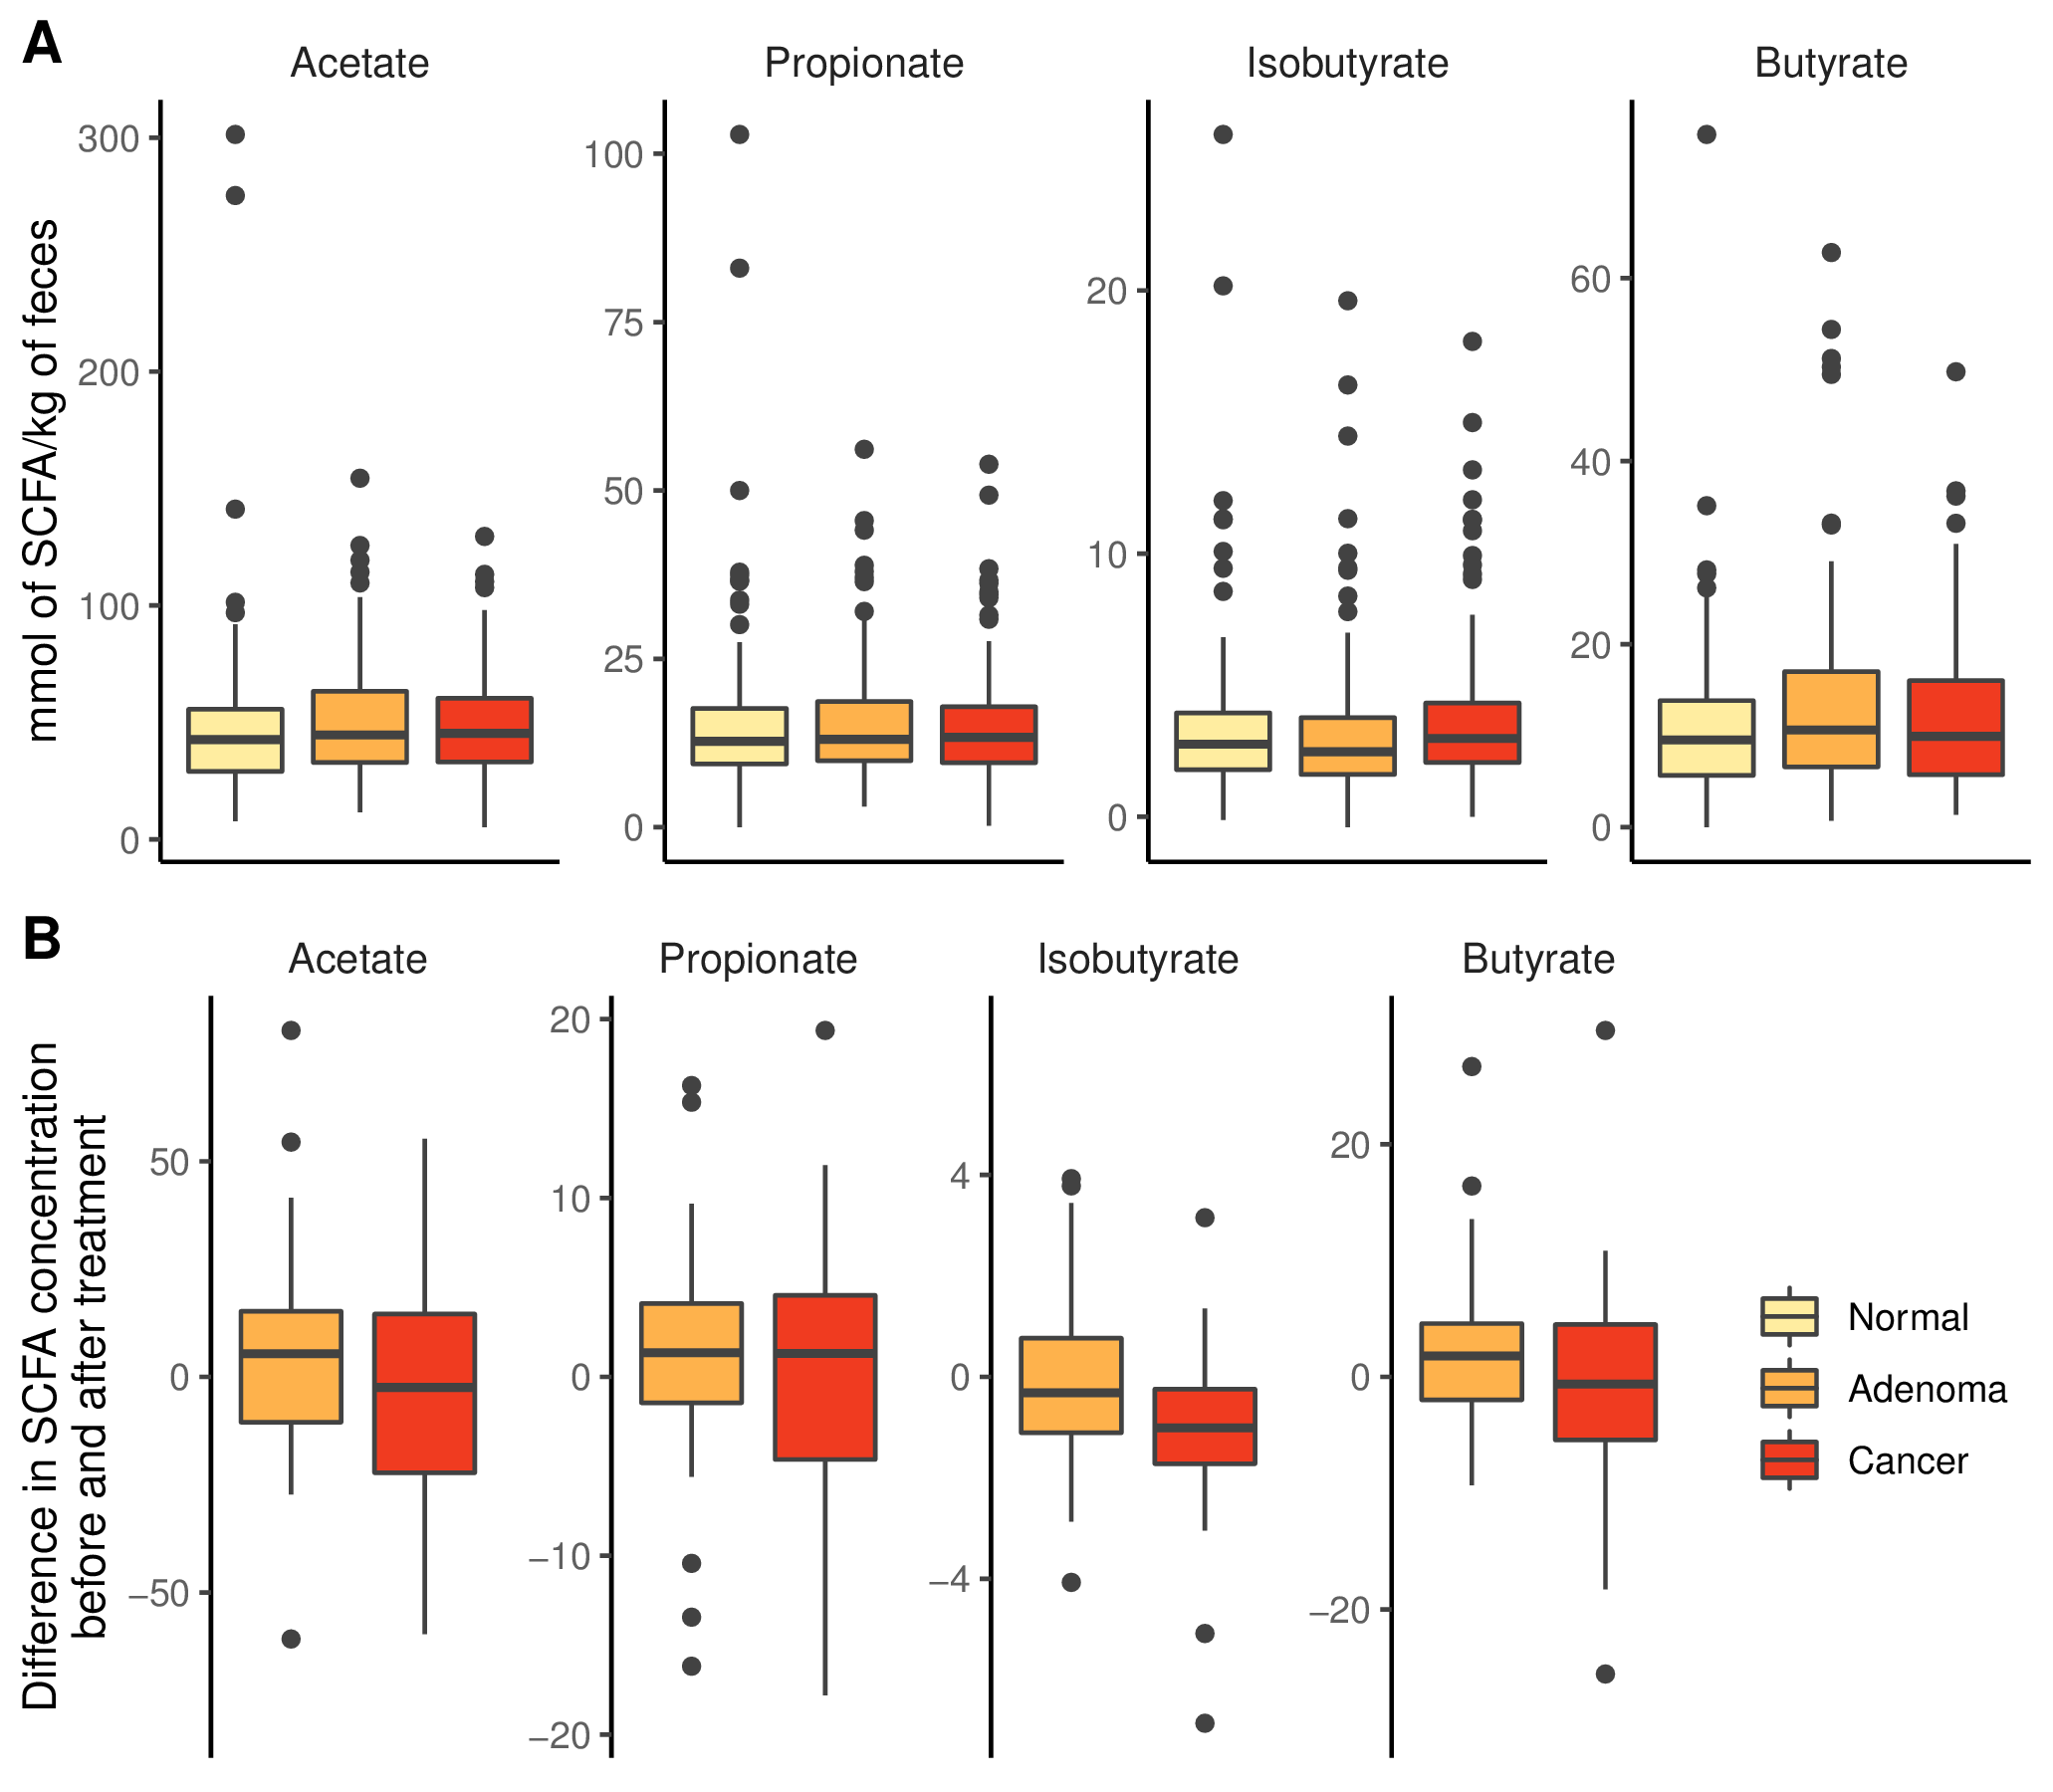
\includegraphics{figure_1.png}

\textbf{Figure 1. SCFA concentrations did not vary meaningfully with
diagnosis of colonic lesions or with treatment for adenomas or
carcinomas.} (A) The concentration of fecal SCFAs from individuals with
normal colons (N=172) or those with adenoma (N=198) or carcinomas
(N=120). (B) A subset of individuals diagnosed with adenomas (N=41) or
carcinomas (N=26) who underwent treatment were resampled a year after
the initial sampling; one extreme propionate value (124.4 mmol/kg) was
included in the adenoma analysis but censored from the visualization for
clarity.

\newpage

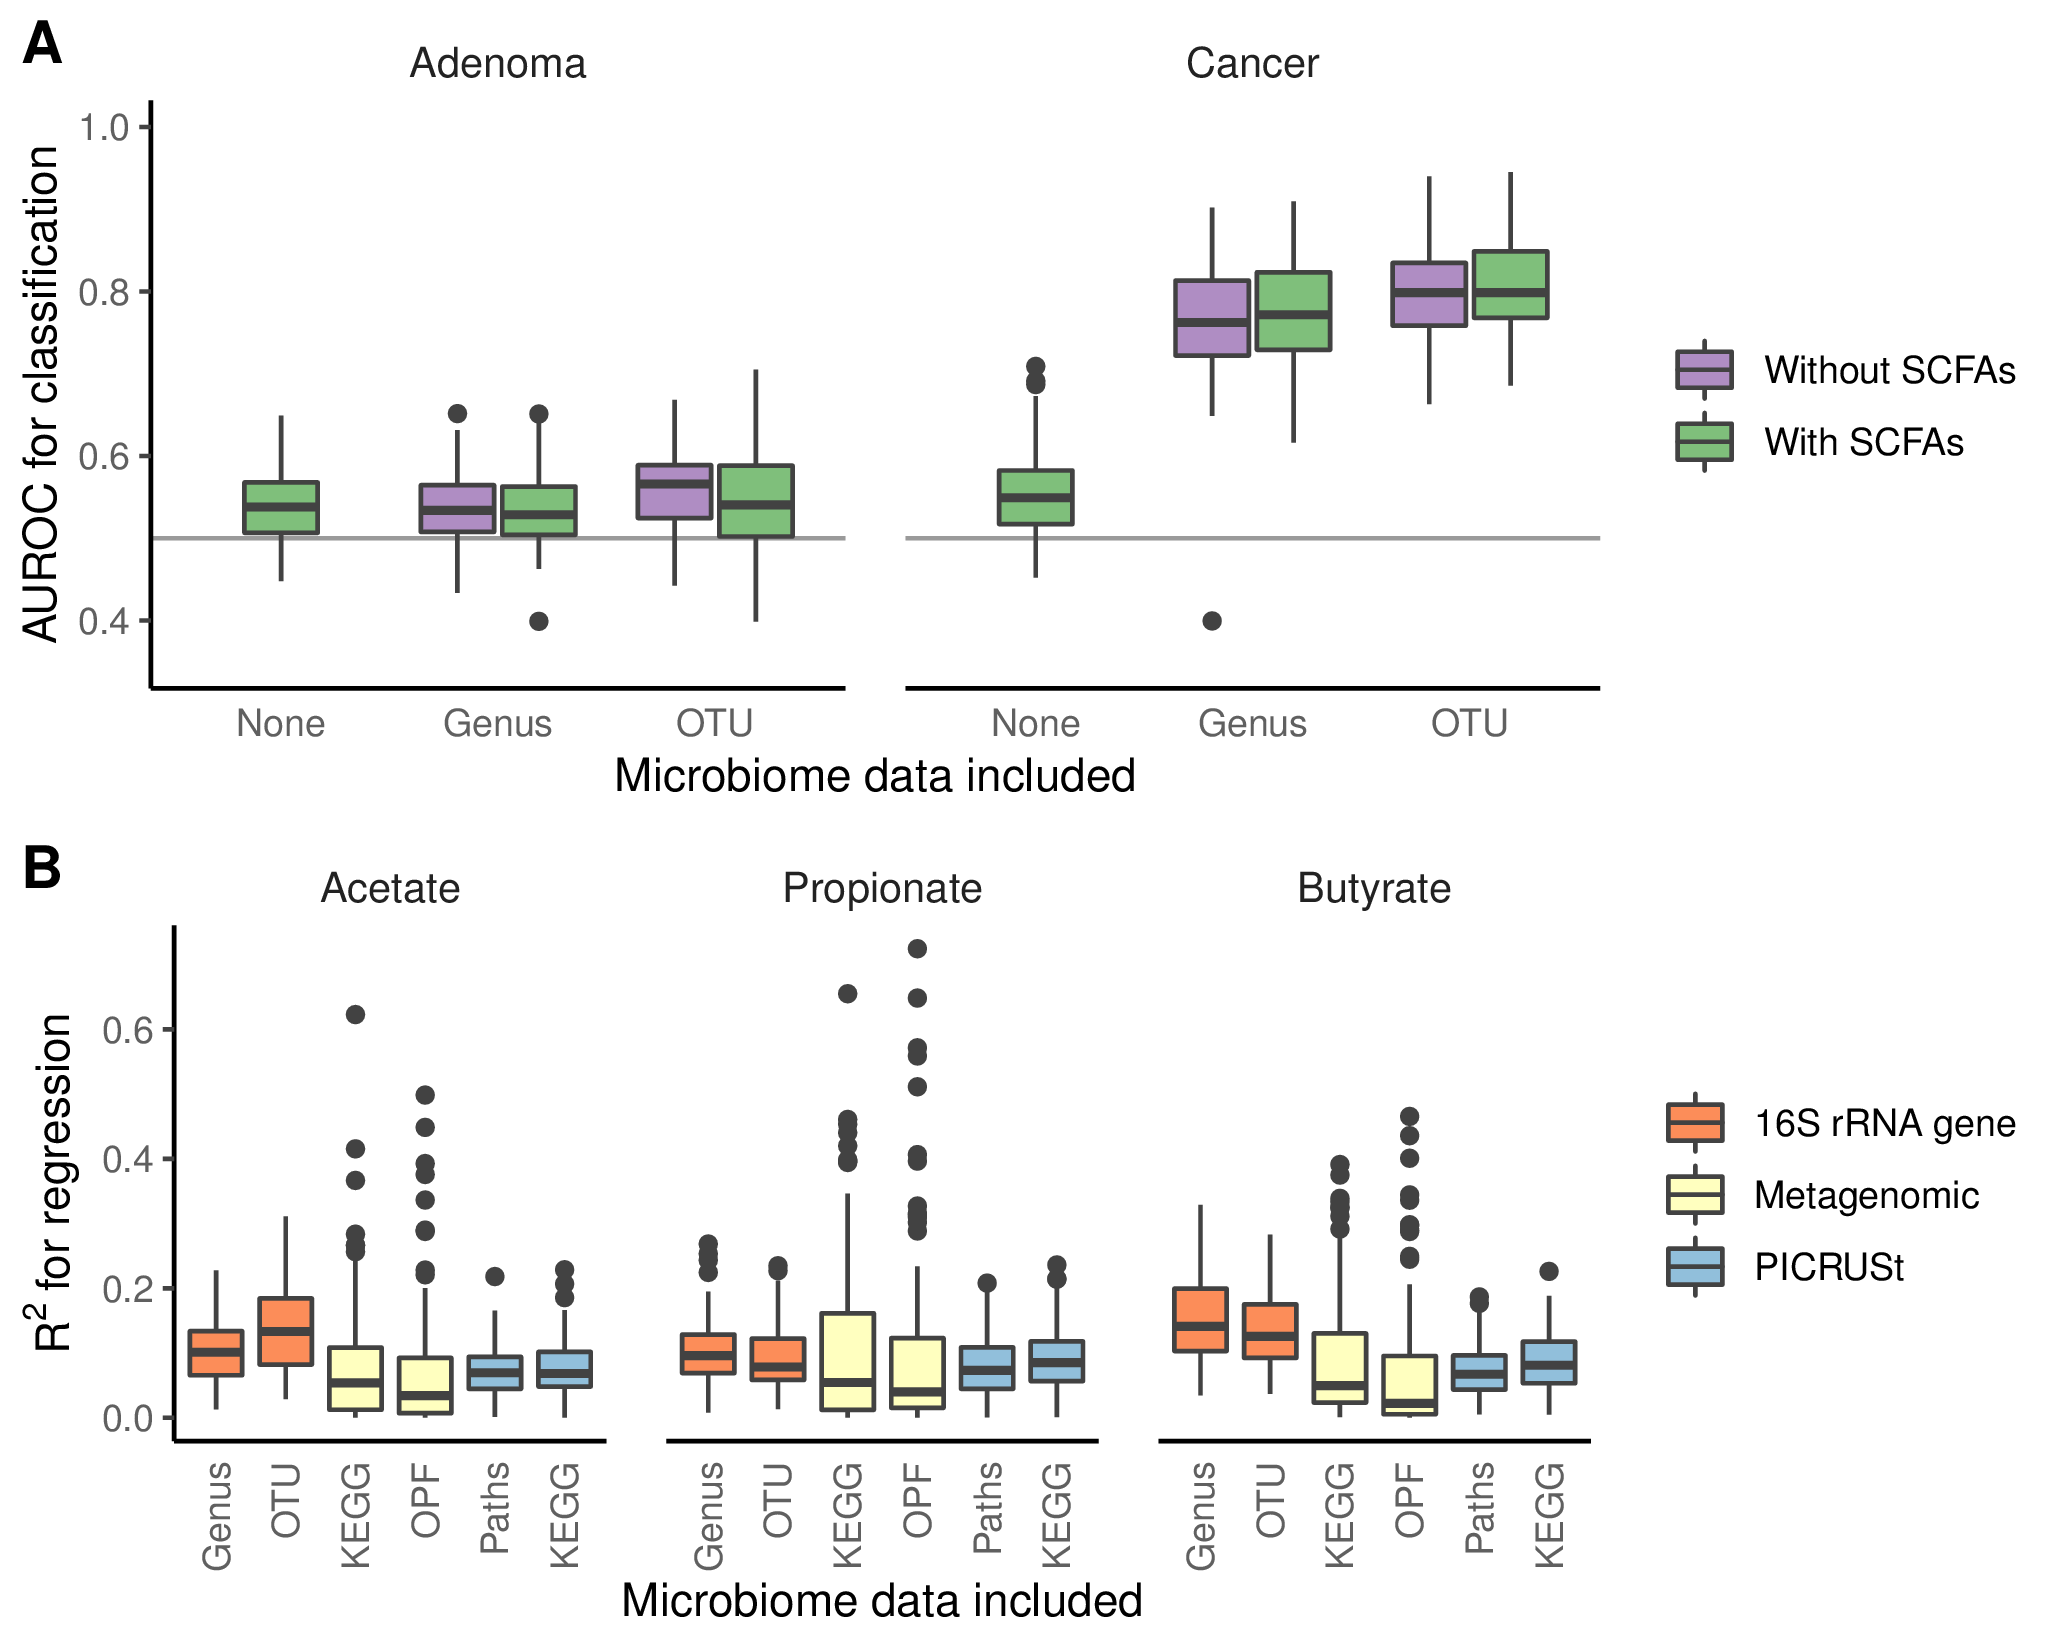
\includegraphics{figure_2.png}

\textbf{Figure 2. SCFA concentrations do not improve models for
diagnosing the presence of adenomas, carcinomas, or all lesions and
cannot be reliably predicted from 16S rRNA gene or metagenomic sequence
data.} (A) The median AUROC for diagnosing individuals as having
adenomas or carcinomas using SCFAs was slightly better than than chance
(depicted by horizontal line at 0.50), but did not improve performance
of the models generated using 16S rRNA gene sequence data. (B)
Regression models that were trained using 16S rRNA gene sequence,
metagenomic, and PICRUSt data to predict the concentrations of SCFAs
performed poorly (all median R\textsuperscript{2} values \textless{}
0.14). Regression models generated using 16S rRNA gene sequence and
PICRUSt data included data from 490 samples and those generated using
metagenomic data included data from 78 samples.

\newpage

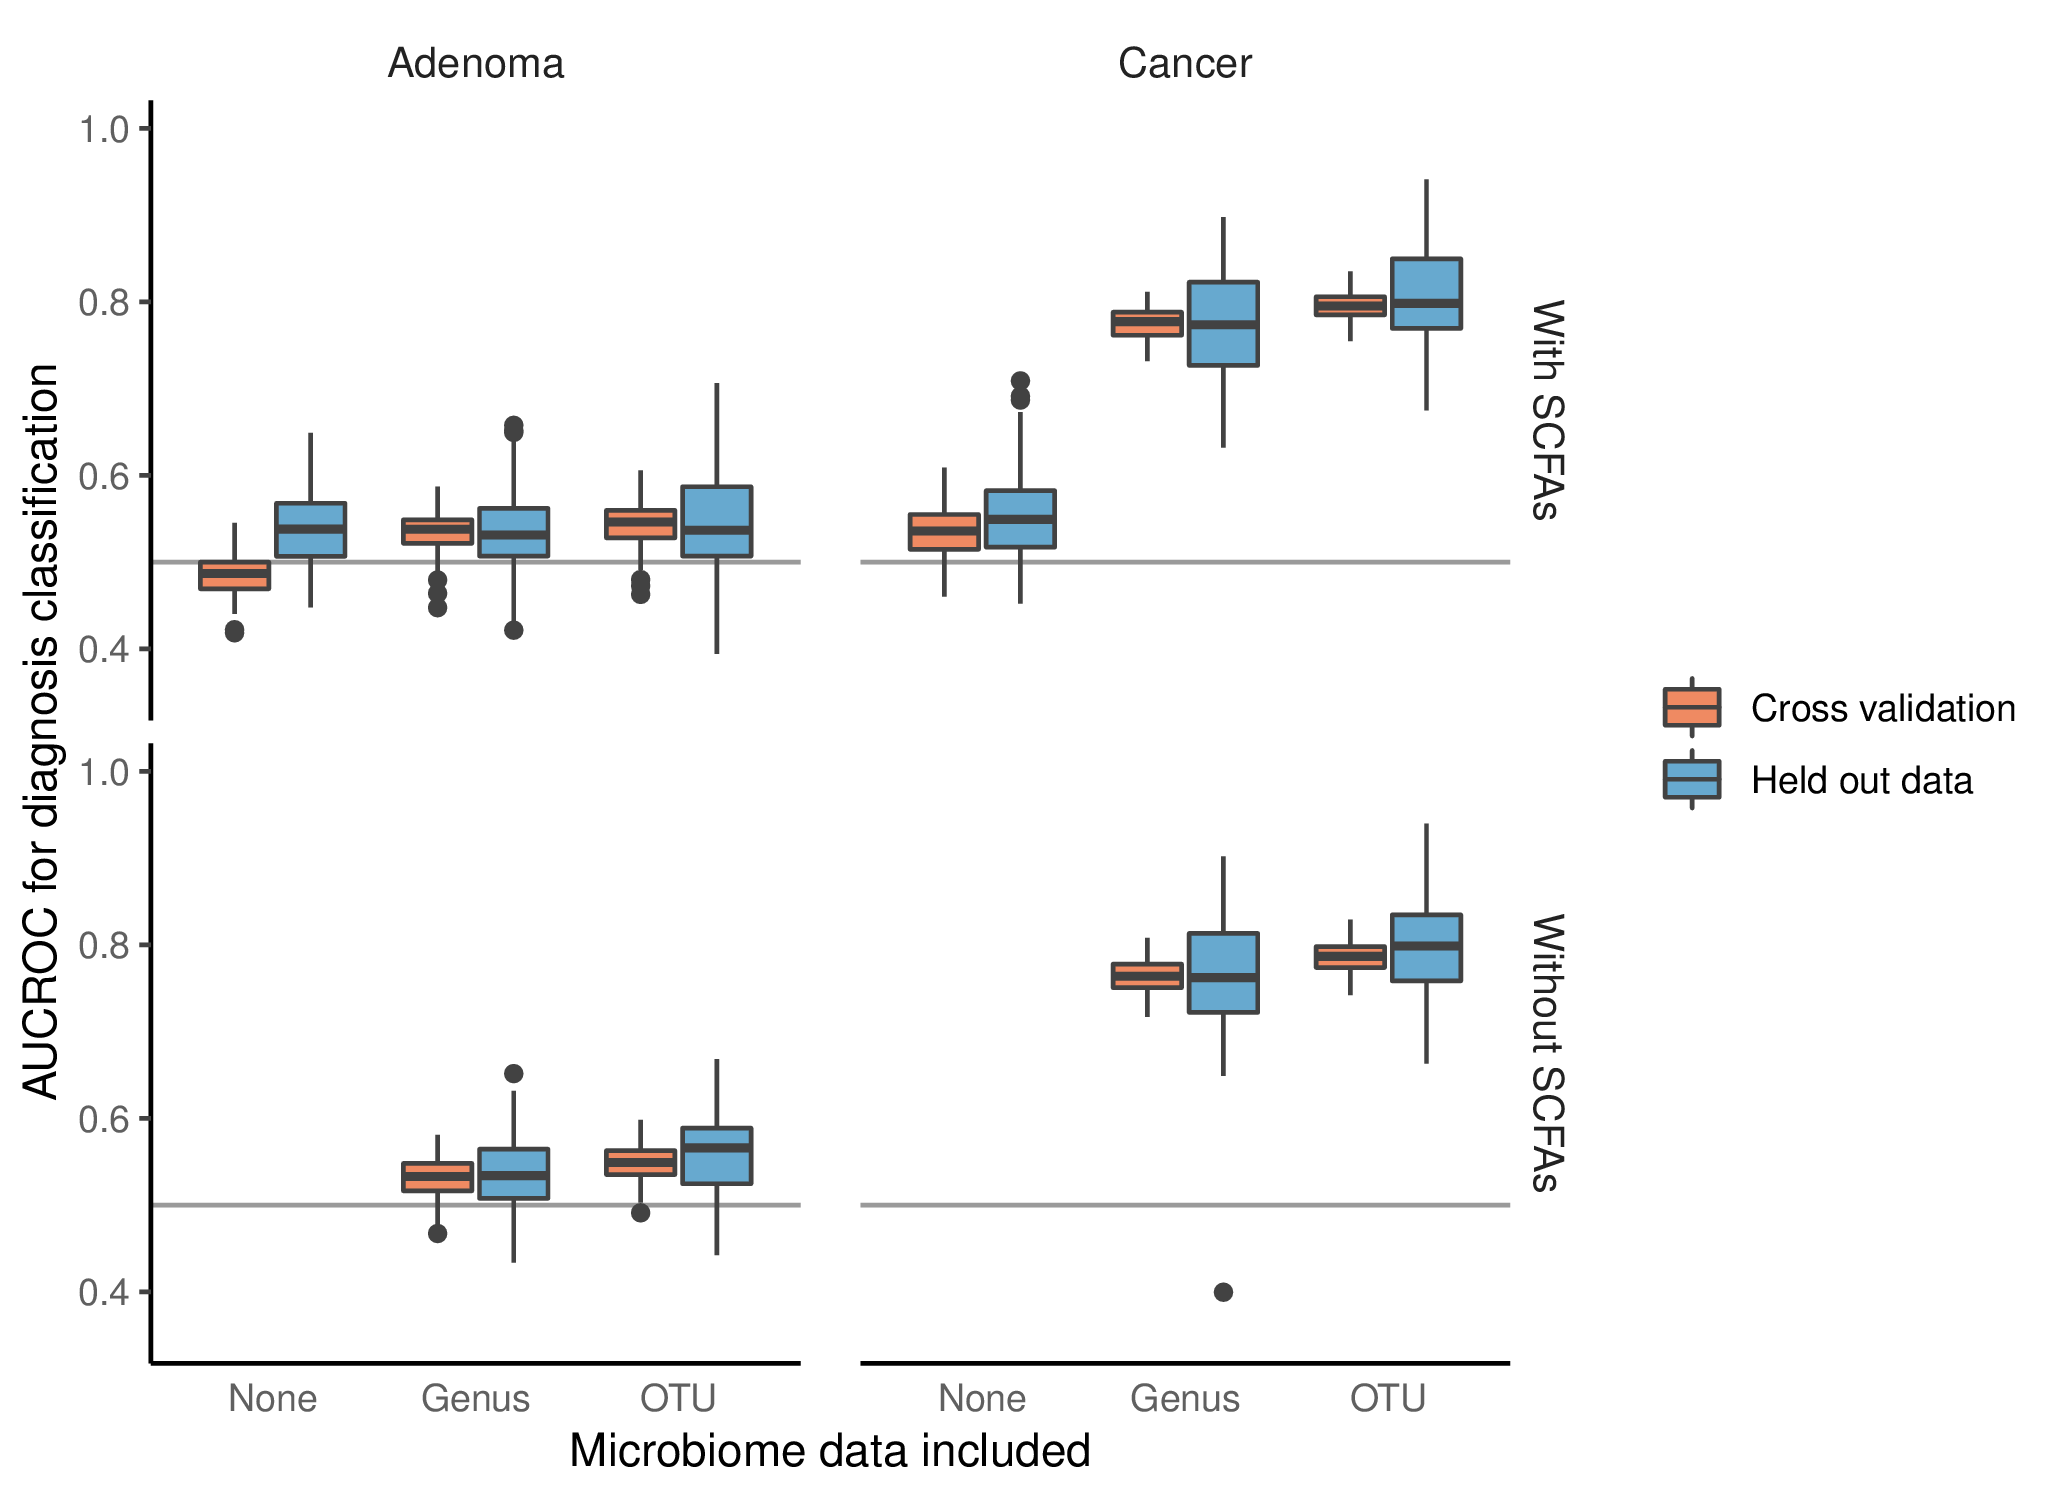
\includegraphics{figure_s1.png}

\textbf{Figure S1. Comparison of training and testing results for
classification models shows that the models are robust and are not
overfit.} random forest classification models were generated to
differentiate between individuals with normal colons and those with
adenomas or carcinomas using 16S rRNA gene sequence data that were
clustered into genera or OTUs with and without including the three SCFAs
as additional features. random forest classification models were
generated by partitioning the samples into a training set with 80\% of
the data and a testing set with the remaining samples for 100
randomizations.

\newpage

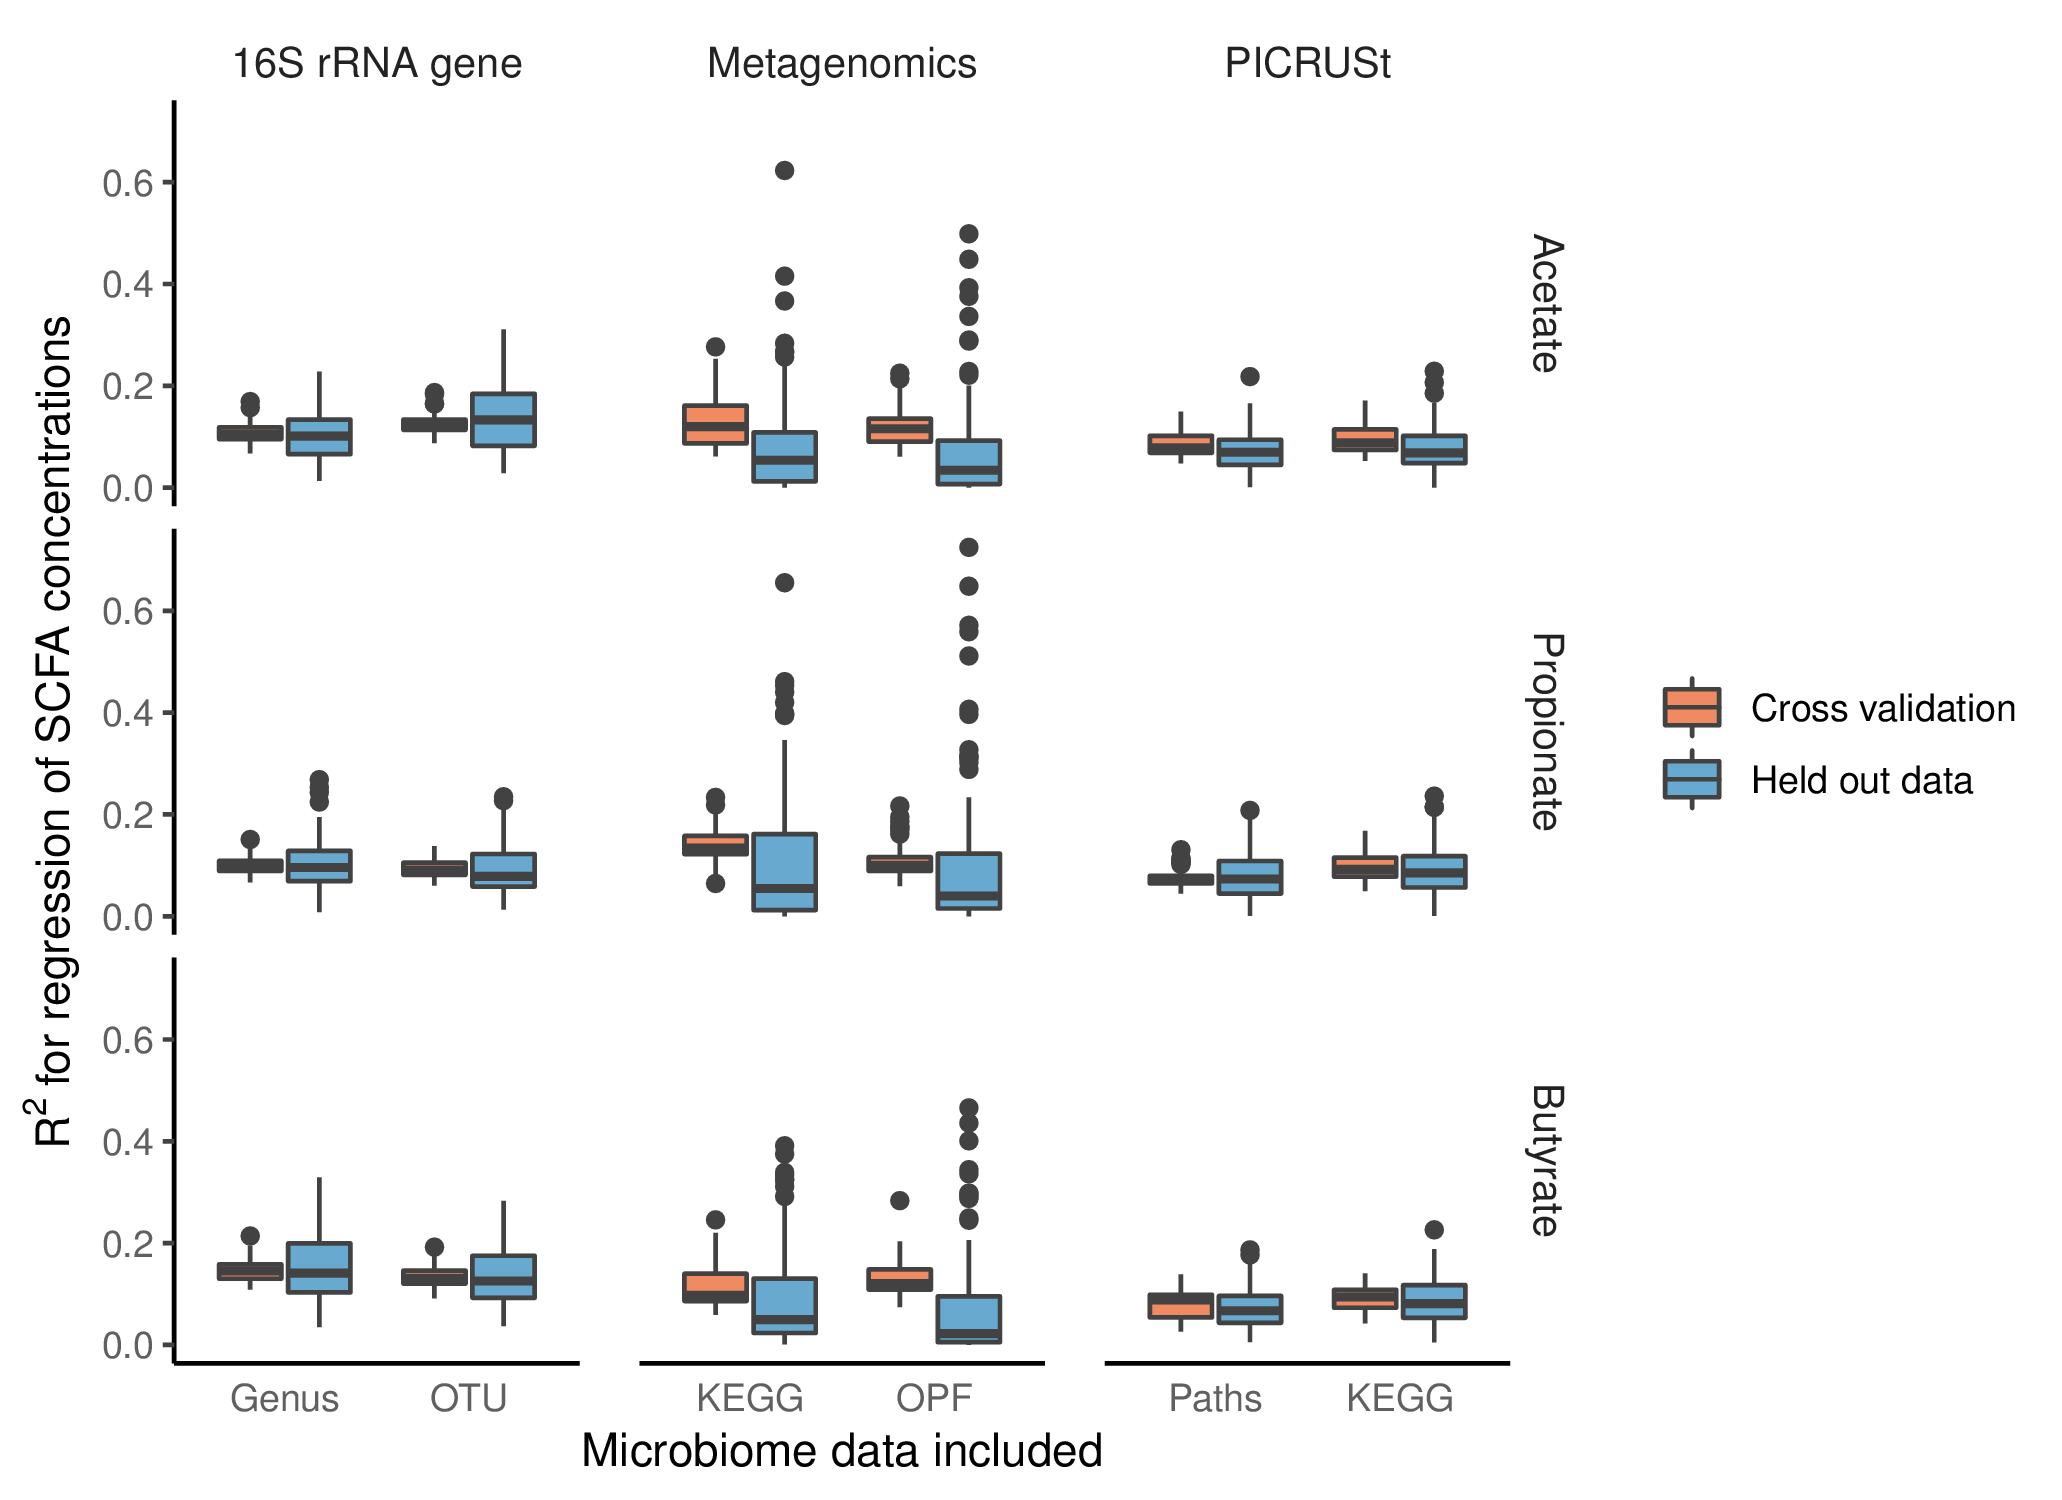
\includegraphics{figure_s2.png}

\textbf{Figure S2. Comparison of training and testing results for
regression models shows that the models are robust and are not overfit.}
random forest regression models were generated to predict the
concentration of each SCFA using each individuals' microbiome data
generated using 16S rRNA gene sequence and metagenomic sequence data.
These regression models were generated by partitioning the samples into
a training set with 80\% of the data and a testing set with the
remaining samples for 100 randomizations.


\end{document}
